% !TeX root = ../main.tex
% Add the above to each chapter to make compiling the PDF easier in some editors.
\chapter{Related Work}\label{chapter:related-work}

\section{Classification of location data and apps that use it}
In order to review existing approaches and research, we classify location aware services by the acceptable delay of the location information being available:
Such a classification has already been made by \parencite{hoh2005protecting}.
\begin{enumerate}
  \item Almost no delation tolerance: e.g. an application showing a pop-up about a nearby venue e.g. a coffe shop when a pedestrian passes
  \item Some delay e.g. one minute is acceptable: An application e.g. google maps derives the information of congested traffic from devices reporting their GPS data which show lower than usual speed. As congestions worth reporting last longer than one minute, some delay in the device's information reaching the server is acceptable.
  \item Significant delay of hours, days or even weeks is acceptable for historical and statistical use of location data e.g. to find out about popular visiting times
\end{enumerate}
Most research investigates user's privacy in case 3 [Citations!!!] or 2. For case one there are already solutions available.
We will first review research tackling location privaacy in case 3 and 2 and then briefly point out the findings for case 1.

%\subsection{What has been achieved so far}

%Most existing approaches focus on publishing location data where a huge delay is acceptable as can be seen in the following table: TODO [create table].

\section{Research has identified the following privacy problems}
\subsection{Central databases itself pose a risk due to possible theft}
%Centralized databases also expose the users to a security risk (through theft of data) \parencite{iot, hoh2006enhancing}.

%\begin{itemize}
%		\item \parencite{p2p-android} proposes the use of P2P over WIFI and Bluetooth to decrease the need of central instances.
%		\item \parencite{crowdsourcing} proposes a secure approach where the raw data is hidden from the central instance but still the aggregated data can be obtained by using encryption methods. This approach is very close to our work. Also \parencite{hoh2006enhancing} is close to our work and uses encryption.
%		\item \parencite{hoh2006enhancing} proposes an approach to handle user authentication.
%	\end{itemize}

\subsection{Inference attacks on published data}

\subsubsection{Inferring home and work location from consecutive data samples}
Research has shown, that even from a location data set that is pseudonymous, i.e. the identifiers have been stripped or anonymized from the data, it is still possible to infer the home location of single users through inference attacks \parencite{krumm, cellphone, privacy-home-work-pairs, hoh2006enhancing, twitter}. The same problem arises when using data collected through crowdsourcing \parencite{crowdsourcing}.

\subsubsection{Inferring identity from home and work location}
Furthermore, this location coordinates can then be combined with publicly available information e.g. reverse map coding of coordinates to addresses and then searching for entries in telephone books to infer the users identity from it's home location \parencite{krumm, privacy-home-work-pairs, hoh2006enhancing}. This identity can then be linked to other sensitive data. This problem also arises in the area of IoT \parencite{iot, hoh2006enhancing}.
Often (though with usually lower probability) also the work address in addition to the home address can be inferred and makes linking the data to identities even easier \parencite{cellphone, privacy-home-work-pairs}.

\subsubsection{Solutions / Countermeasures to prevent inference attacks}
Spatial cloaking: Achieving k-anonymity by dropping data points or perturbing them or dropping all data points around a random point around the home location \parencite{krumm}.
More sophisticated approaches: \parencite{time-to-confusion}

\subsubsection{Problems still after countermeasures}
\begin{itemize}
	\item Data suppression algorithms have only limited success and can only reduce, but not eliminate the risk \parencite{hoh2006enhancing}.

\item{Data is useless if k-anonymity is guaranteed}
Insufficient accuracy / the data set becomes useless \parencite{krumm, cellphone, k-anonymity-old, k-anonymity, k-anonymity-achieving}.

\item{Countermeasures not effective in sparsely populated areas}
Anonymization techniques might score well in densly populated areas or areas with high traffic but poorly in sparsely populated areas especially where a single address can be mapped to a single person or family \parencite{time-to-confusion, location-privacy, hoh2006enhancing} [location-privacy correct paper or cited wrong paper???] or might not work for individuals whos work and home location are further away than average \parencite{privacy-home-work-pairs}.

	\item More advanced privacy breaking algorithms
\item Taking other sources into accouont, e.g. history of location data
Extending the time period over which data is collected generally increases the risk.

\item quasi-identifiers not thought of
\end{itemize}
%\subsection{All methods depend on trust to a third party or the provider itself}
%Still all approaches depend on first centrally collecting the original raw data and then before querying \parencite{k-anonymity} applying anonymization techniques.

%\section{Category 1 location data use: instant}
%\parencite{location-privacy, mix-zones} introduces mix-nodes, that can nevertheless not guarantee privacy and also depnds on a trusted third party.
		Also \parencite{casper} proposes a solution (close to our summary) how to enable privacy for instant use of location data.

%Decentralized methods for data analysis are also motivated from the area of IoT \parencite{iot}.

%TODO: Relate to \parencite{k-anonymity}

%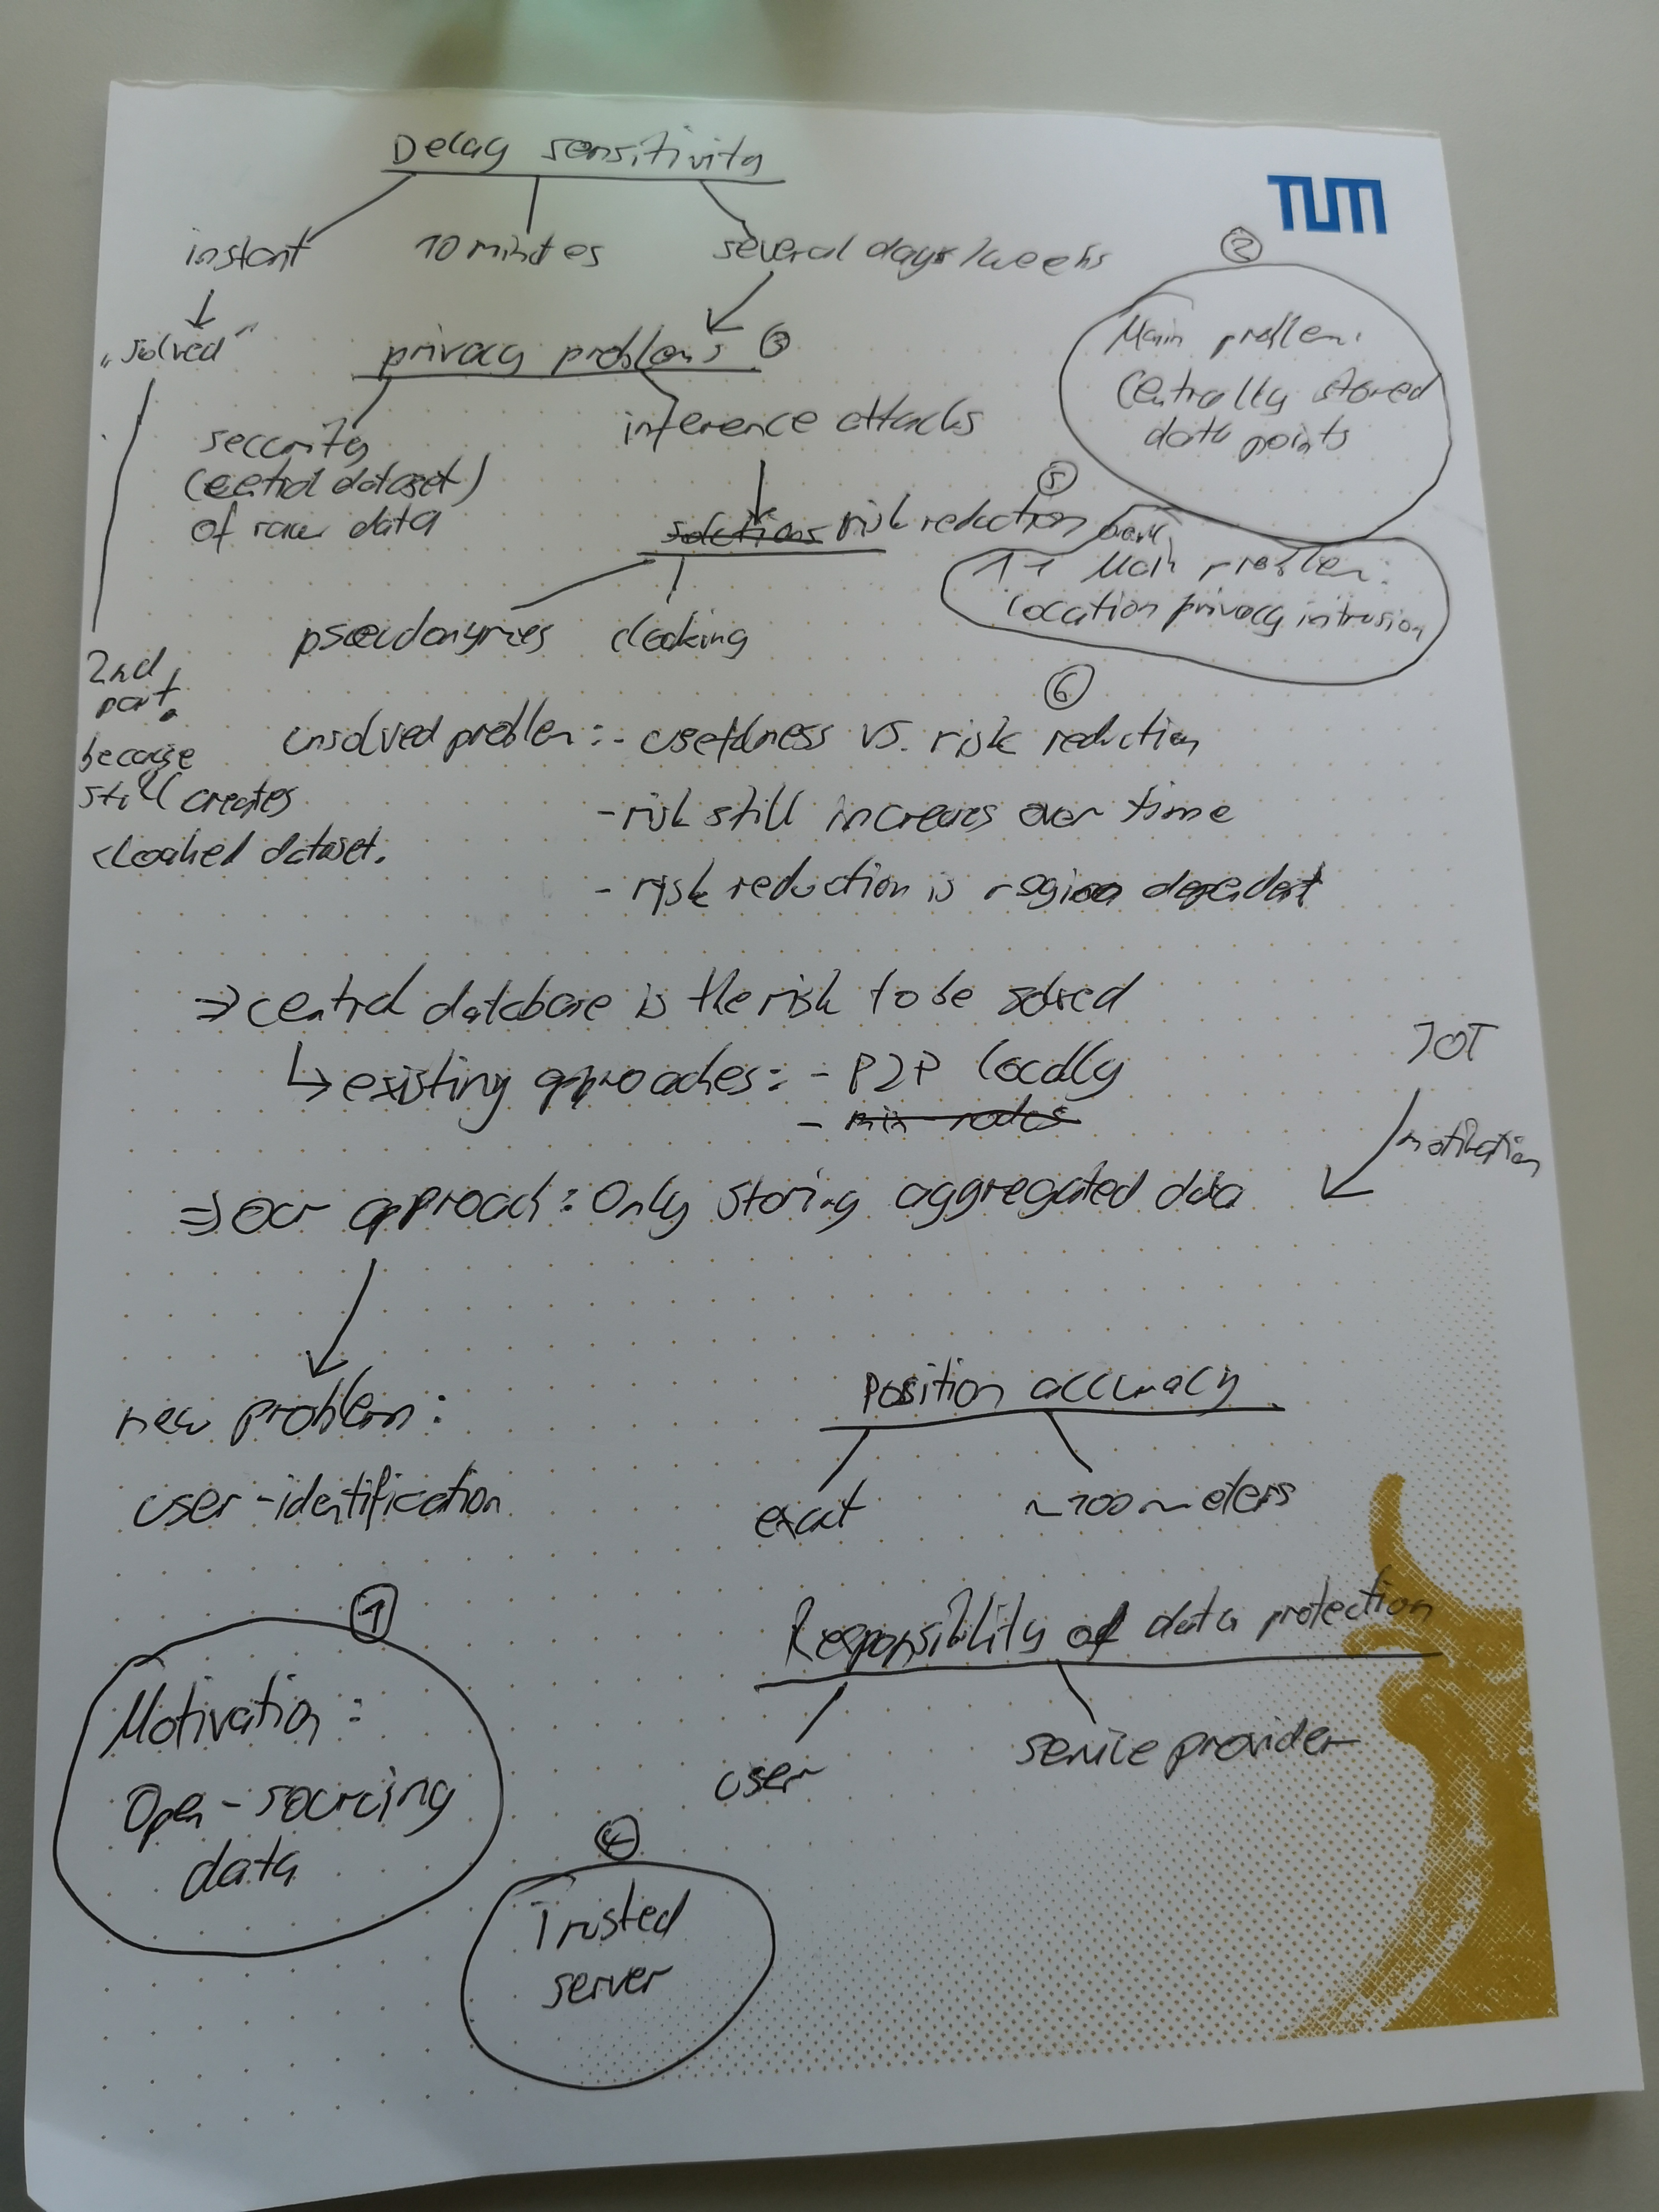
\includegraphics[width=\textwidth]{data/research-overview.jpg}
%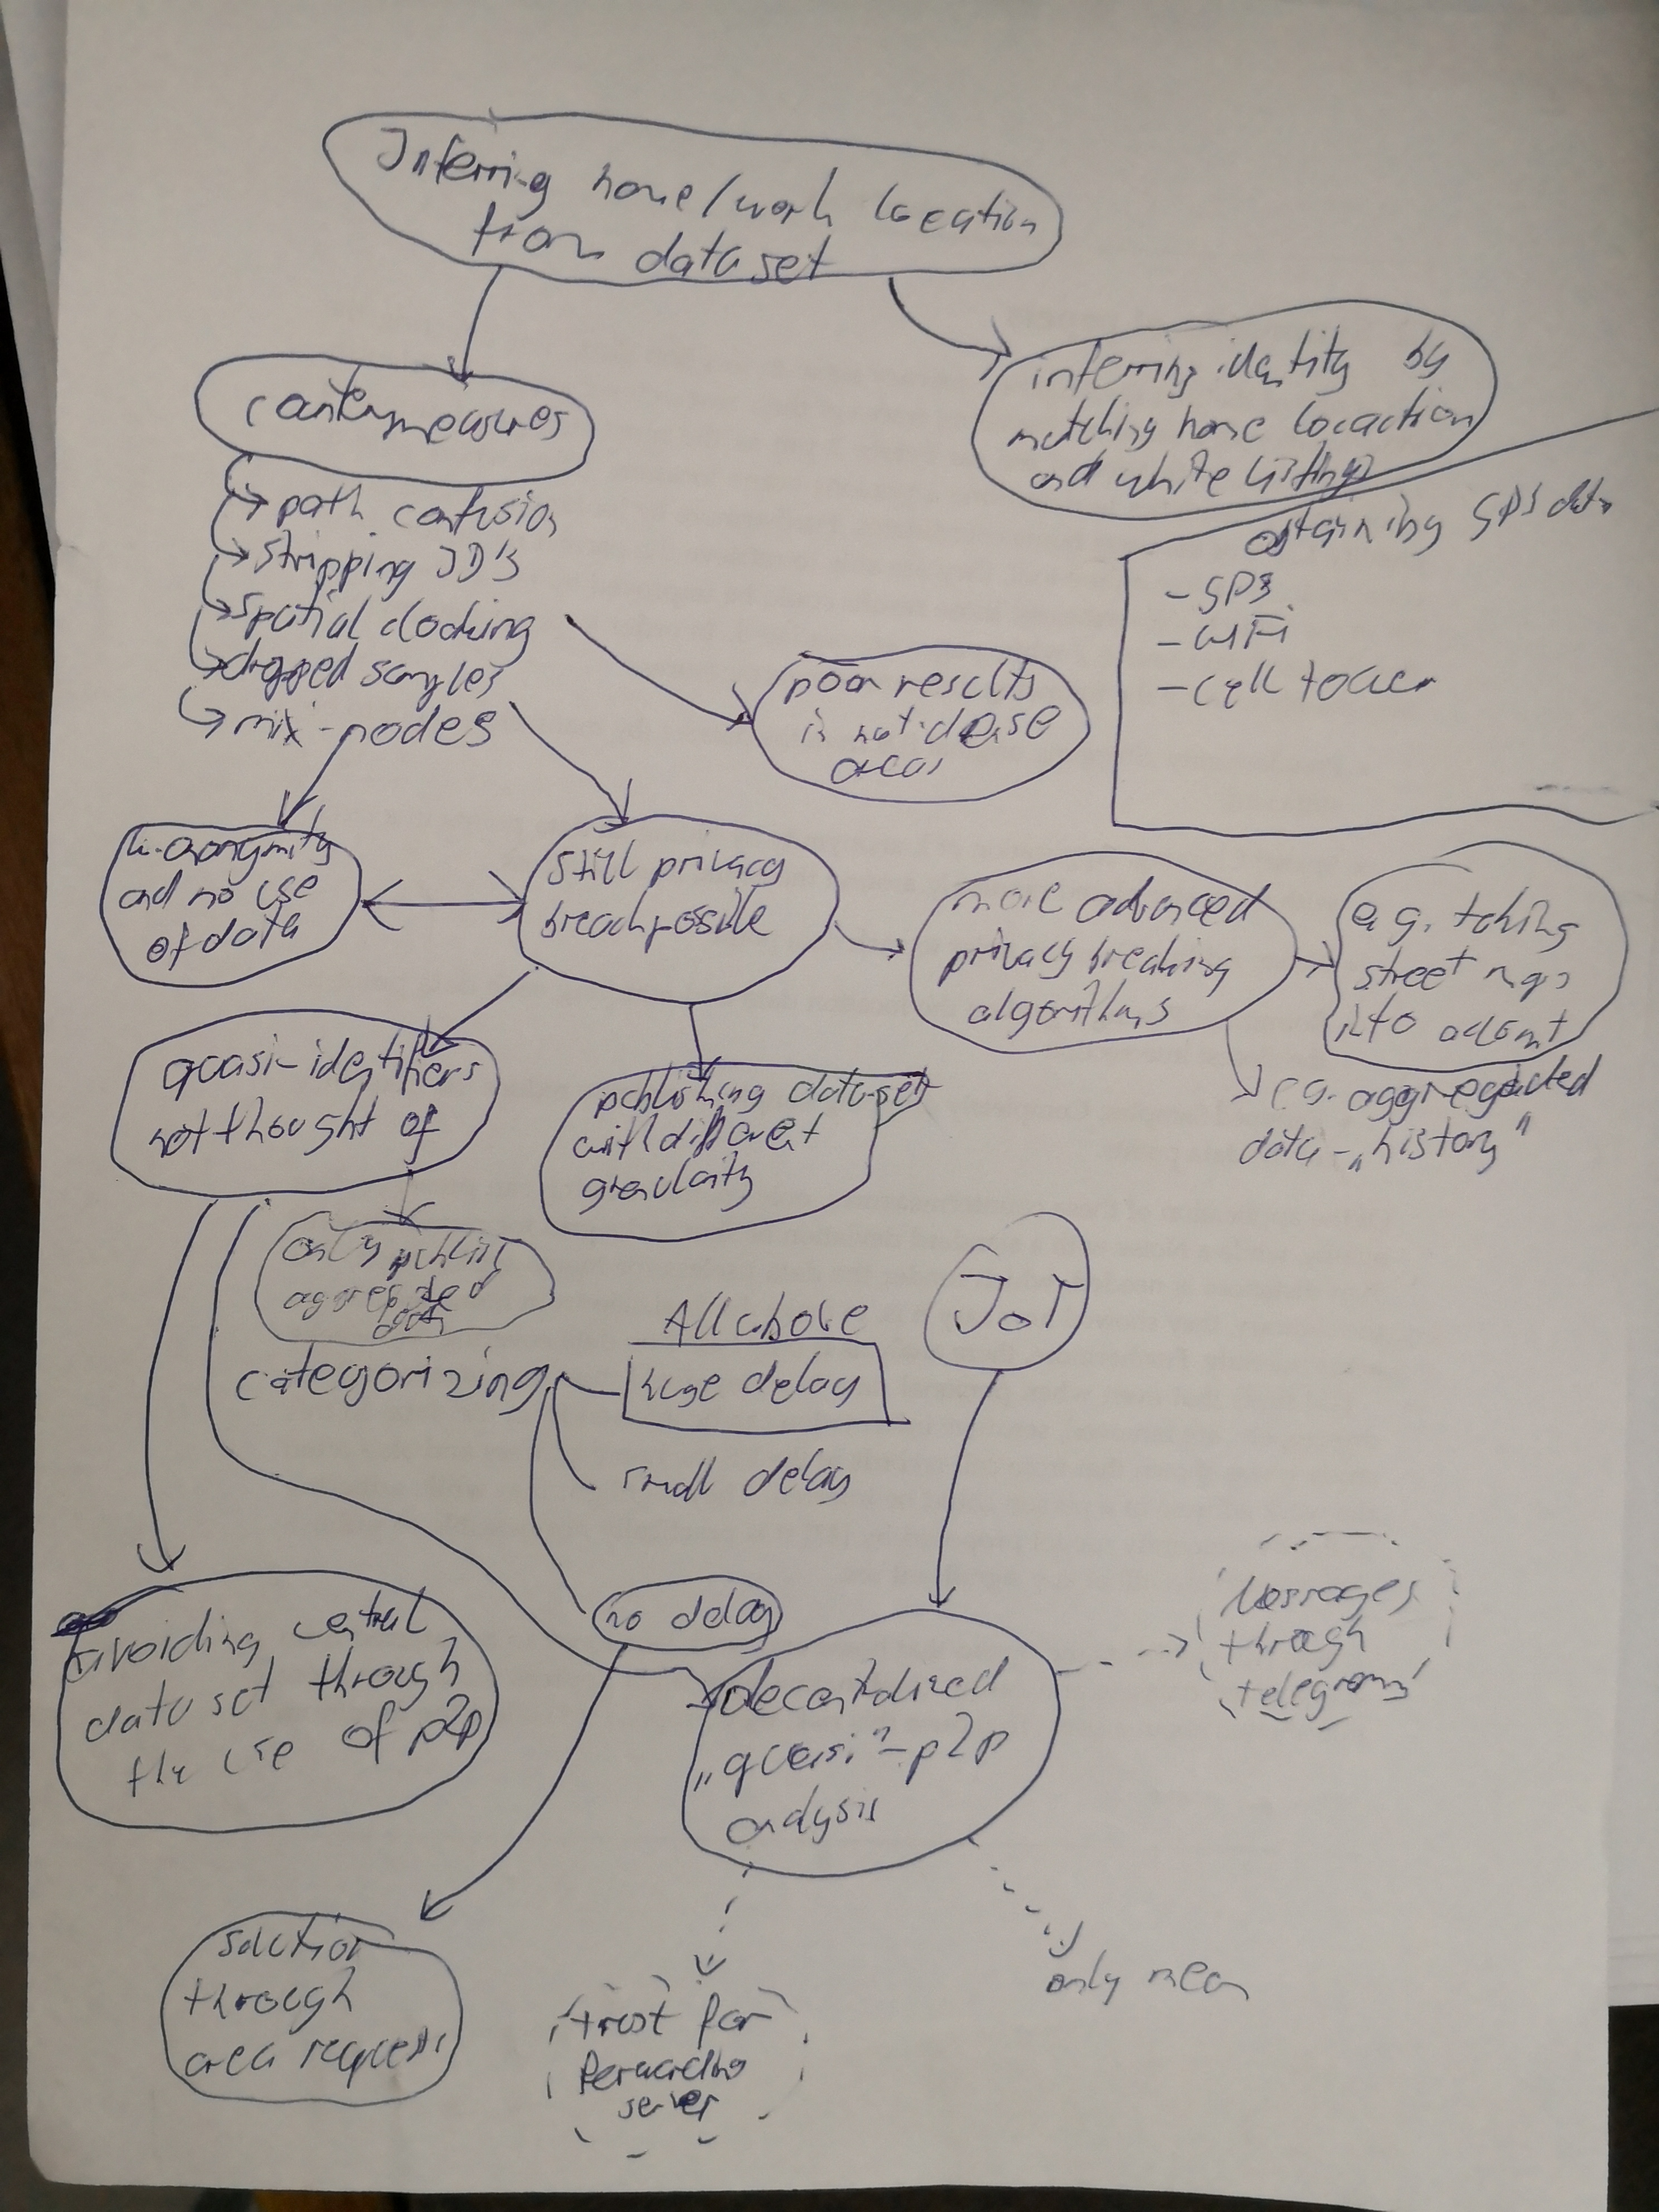
\includegraphics[width=\textwidth]{data/research-overview-2.jpg}
